% This is the main file for the document. It contains the preamble and the document body.，
% The preamble contains the document class, the title, the author, and any packages that are needed.
% 如果需要中文支持,请将 \documentclass{MathNote} 替换为 \documentclass{MathNoteCN}

\documentclass{MathNoteCN}
\usepackage{graphicx}
\usepackage{float} 
\title{报告标题：基于不同模型的卫生资源预测与配置}
\begin{document}

\newcommand{\covertitle}[1]{\begin{center}\Huge\bfseries #1\end{center}}
\newcommand{\coversubtitle}[1]{\begin{center}\Large\bfseries #1\end{center}}
\newcommand{\coverinfo}[1]{\begin{center}\large #1\end{center}}


\thispagestyle{empty} 
\begin{center}
\vspace*{2cm}

% 可选：插入学校/学院logo（需替换图片路径，宽度设为4cm）
% \includegraphics[width=4cm]{school-logo.png}\\[1.5cm] % 图片下方空1.5cm

% 一级标题：课程名称
\covertitle{2025-2026-1 课程设计I-数学模型}
\vspace{1cm} % 空1cm

% 二级标题：大作业序号
\coversubtitle{第一次大作业报告}
\vspace{1.5cm} % 空1.5cm

% 核心标题：作业主题（加粗放大）
\covertitle{基于不同模型的卫生资源预测与配置}
\vspace{3cm} % 空3cm（拉开标题与个人信息距离）

% 个人信息区（左对齐，与标题区错开）
\begin{flushleft}
\large\bfseries 
班级：\underline{2417} \\[0.8cm] % 下划线长度可调整
姓名：\underline{黄宇辰} \\[0.8cm]
学号：\underline{1120243710} \\[0.8cm]
\end{flushleft}

% 底部空出足够距离，可添加日期（可选）
\vfill % 自动填充剩余空间，使底部内容靠下
\coverinfo{提交日期：2025年8月27日} % 可选
\end{center}
\newpage
\begin{figure}[H]
	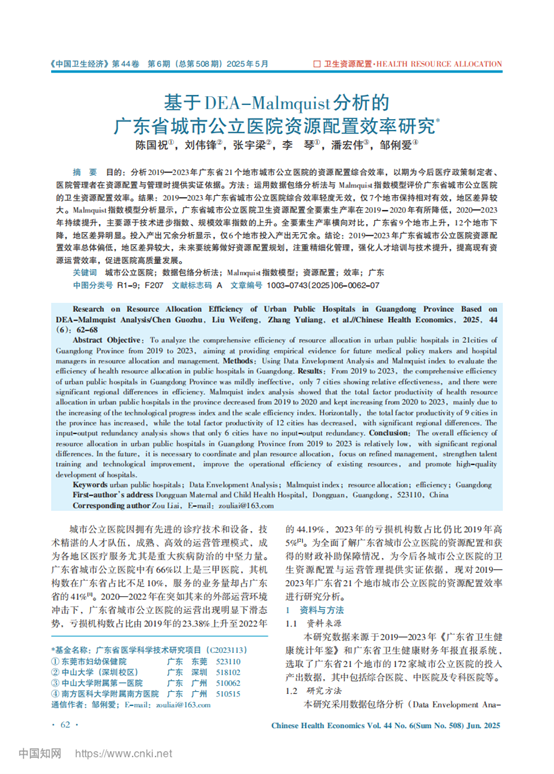
\includegraphics[width=1\textwidth]{cover_1.png}
	\caption{封面1}
	\label{cover_1}
\end{figure}
\newpage
\begin{figure}[H]
	\centering
	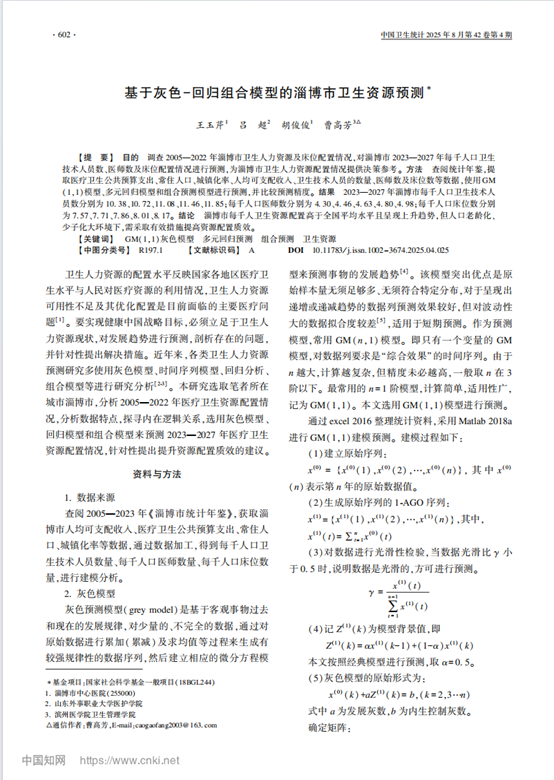
\includegraphics[width=1\textwidth]{cover_2.png}
	\caption{封面2}
	\label{cover_2}
\end{figure}
\maketitle
\section{文献1标题：基于DEA-Malmquist分析的广东省城市公立医院资源配置效率研究}

\subsection{研究问题背景}
城市公立医院作为区域医疗服务核心力量，尤其在重大疾病防治中发挥关键作用。广东省城市公立医院中\textbf{66\%以上为三甲医院}，虽机构数占全省不足10\%，但服务业务量占比达41\%，是当地医疗服务体系的中坚\cite{chen2025}。

2020-2022年受外部运营环境冲击（如公共卫生事件、区域管控政策等），广东省城市公立医院运营显著下滑：亏损机构数占比从2019年的23.38\%升至2022年的44.19\%，2023年亏损占比仍比2019年高5\%\cite{chen2025}。为明确资源配置现状、财政补助保障效果，为政策制定者和医院管理者提供实证依据，本研究聚焦2019-2023年广东省21个地市172家城市公立医院（含综合医院、中医院、专科医院）的资源配置效率，开展系统性分析\cite{chen2025}。


\subsection{模型假设}
1. \textbf{决策单元同质性假设}：广东省21个地市的城市公立医院在运营模式、服务功能（如门诊、住院、手术服务）上具有一致性，投入产出指标的统计口径统一，可作为DEA模型的“决策单元（DMU）”进行横向对比。

2. \textbf{DEA-BCC模型假设}：采用规模报酬变动（Variable Returns to Scale, VRS）假设，即医院资源投入与产出的关系可能随规模扩大呈现递增、不变或递减趋势，符合公立医院在不同发展阶段的实际特征\cite{chen2025}。

3. \textbf{Malmquist指数假设}：假设卫生资源配置的“生产前沿面”可通过历史数据构建，且技术进步具有连续性；全要素生产率（TFP）的变化仅由技术效率（TEC）和技术进步（TC）驱动，暂不考虑极端随机因素（如突发公共卫生事件的短期剧烈冲击）的长期影响\cite{chen2025}。

4. \textbf{数据有效性假设}：研究数据来源于《广东省卫生健康统计年鉴》和卫生健康财务年报直报系统，数据真实、完整，无系统性偏差，可用于投入产出效率测算\cite{chen2025}。


\subsection{数学模型介绍}
本研究采用\textbf{DEA-BCC模型}评价静态效率，结合\textbf{Malmquist指数模型}分析动态全要素生产率。

\subsubsection{DEA-BCC模型}
DEA-BCC模型将综合效率（Overall Efficiency, OE）分解为\textbf{纯技术效率（Pure Technical Efficiency, PTE）}和\textbf{规模效率（Scale Efficiency, SE）}，三者关系为：
\[OE = PTE \times SE\]  
\paragraph{约束}效率值范围为$[0,1]$：效率值=1表示“相对有效”，$0.8 \leq \text{效率值}<1$为“轻度无效”，$0.5 \leq \text{效率值}<0.8$为“中度无效”，效率值<0.5为“严重无效”\cite{chen2025}。  
\paragraph{面向投入的BCC模型线性规划表达式（以第$j_0$个决策单元为例）：}  
  \[
  \begin{cases} 
  \min \theta - \varepsilon \left( \sum_{i=1}^m s_i^- + \sum_{r=1}^s s_r^+ \right) \\
  \sum_{j=1}^n \lambda_j x_{ij} + s_i^- = \theta x_{ij_0} \quad (i=1,2,...,m) \\
  \sum_{j=1}^n \lambda_j y_{rj} - s_r^+ = y_{rj_0} \quad (r=1,2,...,s) \\
  \sum_{j=1}^n \lambda_j = 1 \\
  \lambda_j \geq 0, s_i^- \geq 0, s_r^+ \geq 0 
  \end{cases}
  \]  
  其中，$\theta$为综合效率值，$x_{ij}$为第$j$个单元的第$i$项投入，$y_{rj}$为第$j$个单元的第$r$项产出，$\lambda_j$为权重系数，$s_i^-$（投入冗余）、$s_r^+$（产出不足）为松弛变量\cite{chen2025}。

\subsubsection{Malmquist指数模型}
Malmquist指数用于衡量跨期全要素生产率（TFP）变化，公式分解为：  
\[TFP = TEC \times TC = (PTEC \times SEC) \times TC\]

1. \textbf{TFP（全要素生产率指数）}：>1表示效率提升，<1表示效率下降；

2. \textbf{TEC（技术效率变化指数）}：反映决策单元向生产前沿面靠拢的程度，分解为纯技术效率（PTEC，管理与技术水平）和规模效率（SEC，资源规模合理性）；

3. \textbf{TC（技术进步指数）}：反映生产前沿面的移动，代表诊疗技术、运营模式的创新\cite{chen2025}。


\subsection{求解方法}
\subsubsection{数据来源与指标选取}
1.\textbf{数据来源}：2019-2023年《广东省卫生健康统计年鉴》、广东省卫生健康财务年报直报系统，覆盖21个地市172家城市公立医院\cite{chen2025}。

2.\textbf{投入指标}（人、财、物三维度）：年财政拨款收入（万元）、卫生技术人员数（人）、年固定资产原值（万元）；  

3.\textbf{产出指标}（服务量与效益维度）：门诊诊疗人次（万人次）、出院人次（万人次）、三四级手术量（例）、百元固定资产医疗收入（元）\cite{chen2025}。

\subsubsection{工具与步骤}
1. \textbf{相关性检验}：用Python计算投入-产出指标的Pearson相关系数，验证指标间的线性关联（确保无无关指标干扰）；

2. \textbf{静态效率测算}：用DEAP 2.1软件运行BCC模型，得到21个地市的OE、PTE、SE及投入产出冗余率；

3. \textbf{动态效率分析}：用DEAP 2.1软件构建Malmquist指数模型，分解TFP、TEC、TC、PTEC、SEC的年度与地区差异\cite{chen2025}。


\subsection{求解结果}
\subsubsection{静态效率：综合效率轻度无效，地区差异显著}
1. 2019-2023年广东省城市公立医院综合效率（OE）均值为0.913-0.947，整体呈“轻度无效”；仅佛山、清远、茂名等\textbf{7个地市（占比33\%）}连续5年DEA相对有效，约60\%地市处于轻度无效\cite{chen2025}。

2. 地区分层：粤北地区OE最优（如韶关、梅州），粤东次之，珠三角地区最低（广州、深圳、珠海、肇庆OE持续中轻度无效，肇庆为全省最低）\cite{chen2025}。  

3. 效率分解：纯技术效率（PTE）均值0.954-0.976（轻度无效），47.62\%地市PTE有效；规模效率（SE）均值0.957-0.971（轻度无效），33.3\%地市SE有效，珠三角地区SE偏低（广州、深圳规模报酬递减）\cite{chen2025}。

\subsubsection{动态效率：TFP先降后升，技术进步为核心驱动}
1. 年度趋势：2019-2020年TFP下降（因技术进步指数TC低于均值31\%），2020-2023年TFP持续提升（源于TC和SEC上升）；2022-2023年TFP小幅下降，因PTEC波动\cite{chen2025}。

2. 地区差异：9个地市TFP上升（如梅州，TC和PTEC同步提升），12个地市TFP下降（如汕尾，TC降幅最大）；地市间TFP差异主要源于TC（技术进步）和PTEC（管理水平）\cite{chen2025}。

\subsubsection{投入产出冗余：固定资产与财政补助冗余突出}
1. 仅6个地市无投入产出冗余；14个地市存在投入冗余，主要集中在\textbf{固定资产原值（67\%地市）}和\textbf{财政拨款收入（61\%地市规模报酬递减）}；

2. 产出不足集中在\textbf{百元固定资产医疗收入}（广州、深圳2023年冗余率仍超100\%）、三四级手术量（肇庆、阳江）\cite{chen2025}。


\section{文献2标题：基于灰色-回归组合模型的淄博市卫生资源预测}

\subsection{研究问题背景}
卫生人力资源配置水平直接反映区域医疗卫生服务能力，是实现“健康中国”战略的核心保障。当前卫生资源可用性不足、配置不均衡是主要挑战，需通过趋势预测优化资源规划\cite{wang2025}。

淄博市作为人口密集型城市，2005-2022年卫生资源显著增长（每千人口卫生技术人员从3.89人升至9.84人，增幅152.96\%），且配置水平高于全国平均（人均可支配收入超全国20\%）\cite{wang2025}。但面临\textbf{人口老龄化（城镇化率74.88\%）、少子化}及人口流动（张店区十年人口增长35.74\%）等问题，需预测2023-2027年卫生资源需求，为资源优化配置提供决策支持\cite{wang2025}。


\subsection{模型假设}
1. \textbf{GM(1,1)模型假设}：淄博市卫生资源数据（每千人口卫生技术人员数、医师数、床位数）呈\textbf{单调递增趋势}，原始数据光滑性满足$\gamma<0.5$（可通过累加生成规律性序列）；数据无极端异常值，短期预测中政策、经济等因素的冲击可忽略\cite{wang2025}。

2. \textbf{多元回归模型假设}：卫生资源指标（因变量）与影响因素（自变量）呈\textbf{线性相关}；自变量间无多重共线性（通过P值剔除无意义变量，如城镇化率）；随机误差项$\varepsilon$满足$E(\varepsilon_i)=0$、$D(\varepsilon_i)=\sigma^2$、$cov(\varepsilon_i,\varepsilon_j)=0$（$i≠j$）\cite{wang2025}。

3. \textbf{组合模型假设}：GM(1,1)与多元回归模型的预测结果具有\textbf{互补性}（GM擅长小样本趋势预测，回归擅长量化变量关联）；权重计算基于“均方误差最小”原则，可最大程度利用两类模型的信息\cite{wang2025}。


\subsection{数学模型介绍}
本研究采用\textbf{GM(1,1)灰色模型}、\textbf{多元线性回归模型}，并构建\textbf{加权平均组合模型}，核心公式如下：

\subsubsection{GM(1,1)灰色模型}
1. \textbf{原始序列与1-AGO序列}：  
   原始序列$x^{(0)} = \{x^{(0)}(1), x^{(0)}(2), ..., x^{(0)}(n)\}$（$x^{(0)}(k)$为第$k$年数据）; 1次累加生成序列（1-AGO）$x^{(1)}(k) = \sum_{i=1}^k x^{(0)}(i)$（增强数据规律性）\cite{wang2025}。  

2. \textbf{光滑性检验}：  
   光滑比$\gamma(k) = \frac{x^{(0)}(k)}{x^{(1)}(k-1)}$，当$\gamma(k)<0.5$时，数据满足建模条件\cite{wang2025}。  

3. \textbf{背景值与微分方程}：  
   背景值$Z^{(1)}(k) = 0.5x^{(1)}(k-1) + 0.5x^{(1)}(k)$（$\alpha=0.5$，经典取值）;灰色微分方程$x^{(0)}(k) + aZ^{(1)}(k) = b$（$a$为发展灰数，$b$为内生控制灰数）\cite{wang2025}。

4. \textbf{时间响应函数与还原}：  
   微分方程解为$x^{(1)}(t) = \left(x^{(1)}(1) - \frac{b}{a}\right)e^{-a(t-1)} + \frac{b}{a}$；还原值（预测值）$\hat{x}^{(0)}(t+1) = (1-e^a)\left(x^{(1)}(t) - \frac{b}{a}\right)$\cite{wang2025}。

\subsubsection{多元线性回归模型}
以“每千人口卫生技术人员数”为例，最终模型（剔除无意义变量后）：  
\[y = \beta_0 + \beta_1 x_1 + \varepsilon\]  

$y$为每千人口卫生技术人员数（因变量），$x_1$为人均可支配收入（自变量，$P<0.001$）；实证公式为：
\[y=1.53x_1 + 3.13\]
调整后$R^2=0.99$，拟合优度极高\cite{wang2025}

\subsubsection{加权平均组合模型}
假设GM(1,1)预测值为$\hat{x}_{1t}$，回归预测值为$\hat{x}_{2t}$，组合预测值：  
\[\hat{x}_t = k_1 \hat{x}_{1t} + k_2 \hat{x}_{2t} \quad (k_1 + k_2 = 1)\]

权重$k_1、k_2$按“残差方差倒数”计算，如每千人口卫生技术人员数：$k_1=0.11$，$k_2=0.89$\cite{wang2025}


\subsection{求解方法}
\subsubsection{数据来源与预处理}
\paragraph{数据来源}：2005-2023年《淄博市统计年鉴》，提取常住人口、城镇化率、医疗卫生公共预算支出、人均可支配收入等原始数据，加工为“每千人口卫生技术人员数”“每千人口医师数”“每千人口床位数”3个核心指标\cite{wang2025}。
\paragraph{数据筛选}：多元回归模型中，剔除$P>0.05$的变量（如城镇化率、医疗预算支出），仅保留“人均可支配收入”（2014-2022年数据，确保口径一致）\cite{wang2025}。

\subsubsection{工具与步骤}

1. \textbf{GM(1,1)建模}：用Excel 2016整理数据，Matlab 2018a实现建模与预测；通过\textbf{后验比C}（<0.35为一级精度）和\textbf{小误差概率P}（>0.95为一级精度）验证精度\cite{wang2025}。

2. \textbf{多元回归建模}：用Excel 2016进行线性回归，通过调整$R^2$、F检验（$P<0.001$）验证拟合优度\cite{wang2025}。

3. \textbf{组合模型构建}：计算GM(1,1)与回归模型的残差方差，按“方差倒数”分配权重，生成最终预测值\cite{wang2025}。


\subsection{求解结果}
\subsubsection{单一模型精度均达优级标准}
\paragraph{GM(1,1)模型}：3个指标的后验比$C=0.15-0.26$（<0.35），小误差概率$P=0.98-0.99$（>0.95），均为\textbf{一级精度}\cite{wang2025}。

\paragraph{多元回归模型}：调整$R^2=0.91-0.99$（接近1），F值=77.78-621.95，$P<0.001$，拟合优度\textbf{优}\cite{wang2025}。

\subsubsection{组合模型预测结果：资源持续增长}
2023-2027年淄博市卫生资源预测值（组合模型）如下\cite{wang2025}：  

\begin{table}[h]
\centering
\caption{2023-2027年淄博市卫生资源组合模型预测结果}
\begin{tabular}{|c|c|c|c|}
\hline
年份 & 每千人口卫生技术人员数 & 每千人口医师数 & 每千人口床位数 \\
\hline
2023 & 10.44 & 4.58 & 7.64 \\
\hline
2024 & 10.80 & 4.80 & 7.81 \\
\hline
2025 & 11.19 & 5.03 & 7.98 \\
\hline
2026 & 11.59 & 5.27 & 8.15 \\
\hline
2027 & 12.02 & 5.53 & 8.34 \\
\hline
\end{tabular}
\end{table}

\subsubsection{结论：配置水平领先，但需应对结构挑战}
淄博市每千人口卫生资源配置高于全国平均，但需针对\textbf{老龄化（老年医学人才不足）、少子化（产科/儿科资源调整）、人口流动（张店区资源扩容）}优化结构，推动医养结合、紧密型医联体建设\cite{wang2025}。


\section{文献优缺点对比}
\subsection{模型优势}
\paragraph{文献 1（DEA-Malmquist）}：1. 支持多投入多产出效率评价，贴合医院复杂运营；2. 分解效率维度，定位低效根源；3. 动态分析 TFP 变化，反映长期趋势
\paragraph{文献 2（灰色 - 回归组合）}：1. GM (1,1) 需样本量少，适用数据稀缺场景；2. 组合模型精度高于单一模型；3. 量化经济变量对资源的影响
\subsection{模型局限}
\paragraph{文献 1（DEA-Malmquist）}：1. 对数据同质性要求高，不同区域效率对比存在偏差；2. 动态分析需长期数据支持，短期预测能力有限
\paragraph{文献 2（灰色 - 回归组合）}：1. GM (1,1) 对波动数据拟合差，需样本量多；2. 组合模型精度高于单一模型，计算复杂

\section{改进模型设想与依据}
\subsection{改进方向1：三阶段DEA-Malmquist模型}
\subsubsection{设想}
在文献1的DEA-Malmquist基础上，加入\textbf{环境变量调整阶段}：将“老龄化率”“城镇化率”“人均GDP”作为环境变量，通过SFA（随机前沿分析）剔除环境因素（如珠三角老龄化率低可能提升效率）对原始效率的干扰，再测算“纯净”的技术效率和规模效率，最后结合Malmquist分析动态变化。

\subsubsection{依据}
文献1未考虑外部环境差异（如粤北老龄化率高可能降低OE），导致效率评价存在偏差；三阶段DEA可剥离环境干扰，使地市间效率对比更客观，为政策制定（如向老龄化地区倾斜资源）提供更精准的依据\cite{chen2025}。


\subsection{改进方向2：灰色-回归-ARIMA组合模型}
\subsubsection{设想}
在文献2的灰色-回归组合模型中，加入\textbf{ARIMA模型}（自回归积分移动平均模型）：ARIMA擅长处理波动性数据（如公共卫生事件导致的资源短期波动），将GM(1,1)（趋势预测）、多元回归（变量关联）、ARIMA（波动拟合）的预测值按“熵权法”（综合考虑精度、稳定性）分配权重，生成最终预测结果。

\subsubsection{依据}
文献2的GM(1,1)对波动数据拟合差，而ARIMA可捕捉短期波动；熵权法比“均方误差倒数”更全面（兼顾精度与稳定性），能提升预测抗风险能力，应对人口流动、政策调整等突发因素\cite{wang2025}。
\bibliographystyle{plain}
\begin{thebibliography}{99}
\bibitem{chen2025} 陈国祝, 刘伟锋, 张宇梁, 等. 基于DEA-Malmquist分析的广东省城市公立医院资源配置效率研究[J]. 中国卫生经济, 2025, 44(6):62-68.
\bibitem{wang2025} 王玉芹, 吕超, 胡俊俊, 等. 基于灰色-回归组合模型的淄博市卫生资源预测[J]. 中国卫生统计, 2025, 42(4):602-607.
\end{thebibliography}

		
\end{document}
